\documentclass[10pt,twocolumn]{article}
\usepackage[letterpaper,margin=0.75in,columnsep=0.25in]{geometry}
\usepackage{times}
\usepackage[T1]{fontenc}
\usepackage[utf8]{inputenc}
\usepackage{graphicx}
\usepackage{booktabs}
\usepackage{amsmath,amssymb}
\usepackage{microtype}
\usepackage[round]{natbib}
\usepackage[hidelinks]{hyperref}
\usepackage{caption}
\usepackage{enumitem}
\usepackage{xcolor}

\captionsetup{font=small,labelfont=bf,skip=4pt}
\setlist{nosep,leftmargin=1.1em}
\graphicspath{{../results/figures/}{figures/}}
\newcommand{\lam}{\lambda}
\pagestyle{plain}

\title{\vspace{-2.2em}\textbf{Adaptive Model Selection for LLMs Using Contextual
Bandits}\\[0.2em]\large MSML635 Interim Report --- Group 13}
\author{Amey Hengle \quad Sawyer Byrd \quad Sujeet Madihalli\\
\small University of Maryland, College Park\\
\small \texttt{\{ameyhen, sbyrd1, sujeet\}@umd.edu}\\
\small Code: \url{https://github.com/AmeyHengle/MSML635-Project}}
\date{}

\begin{document}
\maketitle

\begin{abstract}
\noindent
We study LLM routing as a contextual bandit problem, where the router observes
only the outcome of the model it chose and the environment keeps changing. Since
the proposal we have built the full pipeline---a RouterBench stream simulator
with bandit feedback, four scripted shift scenarios, four bandit policies, six
baselines including RouterBench's Zero Router, and three off-policy
estimators---and obtained first results on all three research questions. Three
findings stand out. Linear bandits reach \textbf{96\% of a full-information
supervised router's reward while observing one label per query instead of
eleven}, but clear the Zero Router by only 1.8\%, and $\epsilon$-greedy fails to
clear it at all. Of our four shifts, only the query-mix shift materially harms
the bandits, and the \emph{static} supervised router proves more robust than
they are---the opposite of our hypothesis. Finally, IPS error grows
$3.9\times$ as the logging policy becomes greedier, while SNIPS and DR remain
stable. We also report a blocking dependency problem with the Open Bandit
Pipeline and a miscalibration of $\lam$ that made two of our shift scenarios
no-ops.
\end{abstract}

\section{Problem and Research Questions}

Large language models vary widely in capability and price, and most queries do
not need the most expensive model. A \emph{router} decides, per query, which
model answers. Most academic routers are trained with full-information
labels---obtained by running every model on every query---and evaluated on
static benchmarks \citep{hu2024routerbench,lu2026routerarena}. In deployment
neither assumption holds: a router observes only the outcome of the model it
chose, and models, prices, and traffic keep changing.

At round $t$ a query with features $x_t \in \mathbb{R}^d$ arrives, the router
selects $a_t \in \mathcal{A}$, and observes the reward of that arm only:
\begin{equation}
r(x,a) = \mathrm{quality}(x,a) - \lam \cdot \mathrm{cost}(x,a),
\label{eq:reward}
\end{equation}
with regret measured against the per-query oracle
$a^\star_t = \arg\max_a r(x_t,a)$.

\noindent\textbf{RQ1.} In a stationary setting, how close do bandit routers come
to a supervised router trained with full information?\\
\textbf{RQ2.} Under controlled shifts, do bandit routers adapt faster and
accumulate less regret than a static supervised router?\\
\textbf{RQ3.} Can standard OPE estimators predict a routing policy's value from
logs, checked against simulator ground truth?

\section{Notional Architecture}

Figure~\ref{fig:arch} shows the implemented system. Two design decisions
dominate it.

\textbf{The feedback restriction is a type boundary, not a convention.}
\texttt{BanditEnv.step()} returns a single scalar. The full per-arm reward
vector exists---the oracle, regret, and OPE ground truth all need it---but is
reachable only through \texttt{env.truth}, a separate object handed to the
evaluator and never to a policy. The most damaging available bug in this project
is a policy that accidentally sees rewards it should not, and such a bug
produces beautiful results; making it a structural impossibility was worth the
indirection.

\textbf{$\lam$ is applied downstream of the stream.} The stream emits
\texttt{(quality\_vec, cost\_vec)} separately rather than a scalar reward, so a
single replay serves an entire $\lam$ sweep instead of re-streaming per point on
the cost--quality frontier.

\begin{figure}[t]
\centering
\small
\setlength{\fboxsep}{3pt}
\begin{tabular}{@{}c@{}}
\fbox{\begin{minipage}{0.90\columnwidth}\centering
\texttt{QueryStore} \\ \scriptsize ids, text, cached features, frozen reducer
\end{minipage}}\\[2pt]
$\downarrow$\\[2pt]
\fbox{\begin{minipage}{0.90\columnwidth}\centering
\texttt{Stream} $\leftarrow$ \texttt{ShiftScheduler} \\
\scriptsize emits $(t, x_t)$; S1 arms, S2 prices, S3 mix, S4 degradation
\end{minipage}}\\[2pt]
$\downarrow$\\[2pt]
\fbox{\begin{minipage}{0.90\columnwidth}\centering
\texttt{Policy.select}$(x_t) \rightarrow (a_t, p_t)$
\end{minipage}}\\[2pt]
$\downarrow$\\[2pt]
\fbox{\begin{minipage}{0.90\columnwidth}\centering
\texttt{BanditEnv.step}$(t,a_t) \rightarrow r_t$ \textbf{(scalar only)}\\[1pt]
\scriptsize retains full $r[t,:]$ --- reachable only via \texttt{env.truth}
\end{minipage}}\\[2pt]
$\swarrow$ \hfill $\searrow$\\[2pt]
\fbox{\begin{minipage}{0.42\columnwidth}\centering\scriptsize
\texttt{DecisionLogger}\\ $(x,a,p,r)$
\end{minipage}}
\fbox{\begin{minipage}{0.42\columnwidth}\centering\scriptsize
\texttt{Evaluator}\\ regret $\mid$ frontier $\mid$ OPE
\end{minipage}}
\end{tabular}
\caption{Implemented architecture. One arrow carries a scalar to the policy;
the full reward vector reaches only the evaluator.}
\label{fig:arch}
\end{figure}

\section{Progress So Far}

\paragraph{Dataset layer (complete).} We load the RouterBench 0-shot release
\citep{hu2024routerbench}: 36{,}497 queries $\times$ 11 models, stored wide with
per-model quality, dollar cost, and response columns. The loader coerces the
quality columns (shipped as \texttt{object} dtype), maps the 86 distinct
\texttt{eval\_name} values onto seven benchmark families, excludes MT-Bench
(0.4\% of rows, too small to split---the same reason RouterBench's authors
excluded it), and keeps the undocumented Chinese-language tail \emph{tagged}
rather than dropped. 34 tests pass.

\paragraph{Characterising the pool.} Table~\ref{tab:pool} and
Figure~\ref{fig:pool} establish that this is a genuine routing problem. Cost
spans $72\times$ from \texttt{mistral-7b} to \texttt{gpt-4}, and quality does
not follow cost monotonically: \texttt{codellama-34b} costs $3.8\times$
\texttt{mistral-7b} and scores worse in aggregate. The per-family view is
starker---\texttt{codellama-34b} scores $0.004$ on MMLU and $0.463$ on MBPP, and
\texttt{llama2-70b} $0.028$ on MMLU against $0.545$ on HellaSwag. Mean per-model
rank standard deviation across families is $1.36$, so model \emph{rankings}
reorder by domain. Inter-model quality correlation averages $0.249$. If
orderings were stable, a context-free policy would suffice.

\paragraph{System layer (complete).} Bandit environment with arm registry,
time-varying cost model and shift scheduler; four policies
($\epsilon$-greedy, LinUCB \citep{li2010contextual}, linear Thompson sampling
\citep{agrawal2013thompson}, discounted LinUCB \citep{russac2019weighted});
six baselines; IPS, SNIPS and doubly robust estimators
\citep{dudik2011doubly}; replay runner with propensity logging.

\paragraph{Verification.} Table~\ref{tab:verif} reports the five checks from the
proposal. The one we consider strongest is (ii): our recomputed oracle agrees
with the \texttt{oracle\_model\_to\_route\_to} column RouterBench ships at
$100\%$ on every answerable query, so the reward bookkeeping is validated
against the benchmark's authors rather than against ourselves.

\begin{table}[t]
\centering\footnotesize
\begin{tabular}{lrrrr}
\toprule
Model & Quality & Cost (USD) & $\times$cheap & Oracle \% \\
\midrule
\texttt{mistral-7b} & 0.306 & 4.56e-05 & 1.0 & 32.0 \\
\texttt{wizardlm-13b} & 0.431 & 7.26e-05 & 1.6 & 23.1 \\
\texttt{mixtral-8x7b} & 0.547 & 1.34e-04 & 2.9 & 16.9 \\
\texttt{codellama-34b} & 0.202 & 1.71e-04 & 3.8 & 1.3 \\
\texttt{yi-34b} & 0.647 & 1.85e-04 & 4.0 & 14.6 \\
\texttt{llama2-70b} & 0.328 & 2.02e-04 & 4.4 & 1.9 \\
\texttt{claude-instant} & 0.598 & 2.31e-04 & 5.1 & 4.4 \\
\texttt{gpt-3.5-turbo} & 0.619 & 2.42e-04 & 5.3 & 3.0 \\
\texttt{claude-v1} & 0.630 & 2.12e-03 & 46.6 & 0.6 \\
\texttt{claude-v2} & 0.636 & 2.40e-03 & 52.7 & 0.6 \\
\texttt{gpt-4} & 0.781 & 3.25e-03 & 71.3 & 1.7 \\
\bottomrule
\end{tabular}
\caption{The eleven-model pool, ordered by mean per-query cost
($n=4{,}982$). Oracle \% is the share of queries the per-query oracle assigns
to that arm at $\lam=10$. Cost spans $72\times$; quality does not follow it.}
\label{tab:pool}
\end{table}

\begin{table}[t]
\centering\small
\begin{tabular}{@{}llc@{}}
\toprule
Check & Evidence & Status \\
\midrule
(i) reward/regret units & unit tests, $\lam$ monotone & pass \\
(ii) oracle correctness & 100\% vs shipped column & pass \\
(ii) nothing beats oracle & min margin $\ge -10^{-12}$ & pass \\
(iii) LinUCB sublinear & 2nd/1st-half ratio $0.197$ & pass \\
(iv) IPS unbiased & bias $-0.019$, RMSE $0.026$ & pass \\
(v) splits disjoint & 34 dataset tests & pass \\
(v) frontier vs RouterBench & qualitative only & partial \\
\bottomrule
\end{tabular}
\caption{Verification status. (iii) and (iv) run on the synthetic stream with
known parameters, which RouterBench cannot provide.}
\label{tab:verif}
\end{table}

\begin{figure*}[t]
\centering
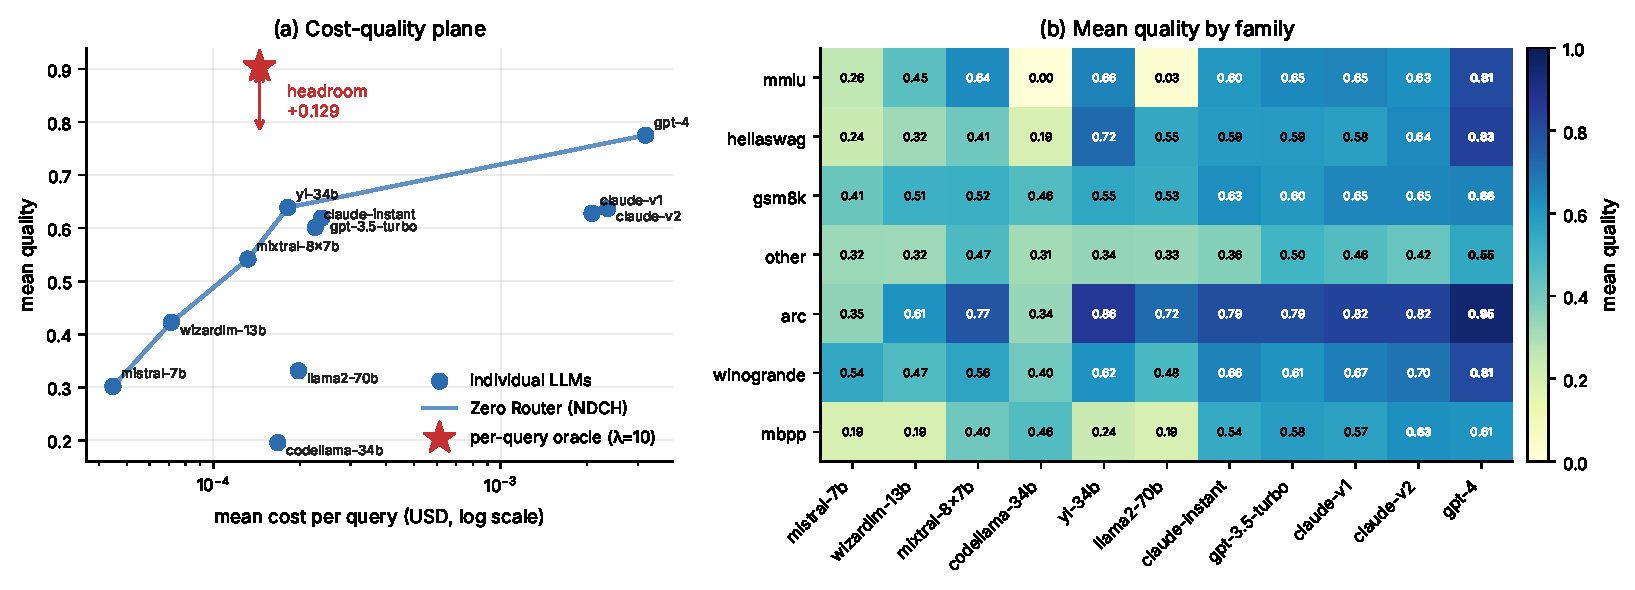
\includegraphics[width=0.92\textwidth]{fig1_pool_and_oracle.pdf}
\caption{(a) The cost--quality plane: eleven models, the non-decreasing convex
hull they span (the Zero Router, AIQ $=0.698$, spanned by only five arms), and
the per-query oracle. The vertical gap is the headroom available to a router.
(b) Mean quality by family: rankings reorder across domains, which is the signal
a contextual router exploits.}
\label{fig:pool}
\end{figure*}

\section{Issues Faced}

\paragraph{Solved: OBP is unusable on the critical path.} Our proposal named the
Open Bandit Pipeline \citep{saito2021open} as our primary base. It declares
\texttt{requires-python >=3.8,<3.11}; on Python 3.13 \texttt{pip} silently
resolves to the much older \texttt{obp 0.4.1} rather than erroring, and when it
does resolve it pulls PyTorch plus the full CUDA toolchain---several
gigabytes---for estimators that are closed-form expressions of roughly thirty
lines. We implemented IPS, SNIPS and DR directly, removing a hard Python ceiling
and a 4\,GB dependency. OBP is retained only in a separate pinned Python 3.10
environment to cross-check our implementations.

\paragraph{Solved: $\lam$ had no calibrated scale.} Equation~\ref{eq:reward} as
written in the proposal left $\lam$ dimensionless. With cost normalised by the
maximum per-query cost, the trade-off is \emph{inert} for $\lam \lesssim 2$: the
oracle's arm distribution is essentially unchanged across $\lam \in [0.1, 5]$.
The frontier bends over $\lam \in [2,30]$ (Figure~\ref{fig:lambda}); at
$\lam=30$ the oracle spends $52\%$ of its $\lam{=}0$ cost while retaining
$97.6\%$ of its quality. Our experiment grid is therefore
$\{0,1,2,5,10,15,20,30,50\}$, not $[0,1]$. At $\lam=0$ the oracle is degenerate:
six arms tie on average.

\paragraph{Solved: our first shift design produced four no-ops.} We initially
targeted S1/S2/S4 at GPT-4 and the cheapest arm. At $\lam=10$ the oracle selects
neither often, so every scenario left all policies statistically
indistinguishable. A shift only tests adaptation if it changes the arm a good
policy would have chosen; the scenarios are now aimed at the oracle's workhorse
arm. S1 and S3 now bite (Section~\ref{sec:rq2}); S2 and S4 still do not.

\paragraph{Solved: LinUCB cannot generate valid logs.} LinUCB is a deterministic
$\arg\max$, so its propensity is identically 1 and IPS degenerates. RQ3
therefore requires its own logging runs with a stochastic policy; it cannot
reuse RQ1/RQ2 logs. \texttt{DecisionLog.check\_loggable()} now raises rather
than silently returning nonsense.

\paragraph{Corrected assumption: rewards are not binary.} We expected quality to
be $0/1$ and flagged the mismatch with LinUCB's linear-Gaussian assumption as a
risk. Measured, $20.6\%$ of (query, model) cells take fractional values
(predominantly $0.25$, $0.5$, $0.75$). The concern was overstated.

\paragraph{Unsolved: recovery time does not discriminate.} Our
proposed metric---rounds until reward returns within 5\% of its pre-shift
level---returns $0$ for every policy in every scenario, because post-shift
reward is already within tolerance on a $200$-round smoothing window. The metric
needs either a tighter tolerance or a per-arm formulation.

\paragraph{Unsolved: features and scale.} Results below use TF-IDF character
$n$-grams reduced by truncated SVD rather than the sentence-transformer
embeddings of the proposal. The character-$n$-gram choice is defensible given
the Chinese-language tail, but the comparison is not yet run. All results are on
a $4{,}982$-query subsample; the loader reads the full release unchanged.

\begin{figure}[t]
\centering
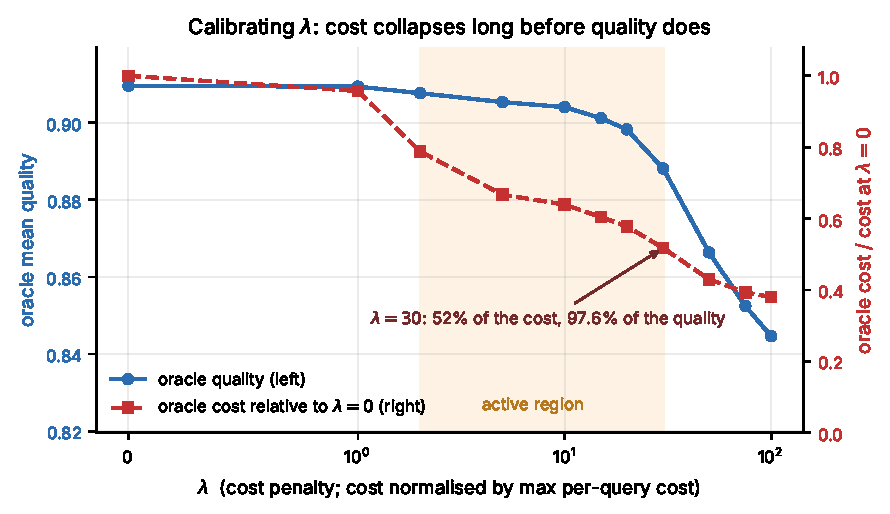
\includegraphics[width=\columnwidth]{fig2_lambda_calibration.pdf}
\caption{Calibrating $\lam$. The cost--quality trade-off is inert below
$\lam \approx 2$ and bends over $[2,30]$.}
\label{fig:lambda}
\end{figure}

\section{Baselines and State of the Art}

\paragraph{Implemented baselines.} \emph{Per-query oracle} (upper bound);
\emph{always-cheapest} and \emph{always-premium}; \emph{uniform random};
\emph{Zero Router}, RouterBench's query-agnostic probabilistic mixture over the
non-decreasing convex hull; \emph{full-information supervised router}, a per-arm
ridge regression trained on calibration data with every arm's reward---the
labelling regime most academic routers assume, and the reference point for RQ1;
and a \emph{confidence-based cascade} \citep{chen2023frugalgpt}, evaluated
directly over the full matrices since it pulls several arms per query.

The Zero Router deserves emphasis because our proposal omitted it.
RouterBench's authors found their own KNN and MLP routers failed to beat it
consistently, so it, not the trivial fixed policies, is the bar. On our data it
is spanned by only five of eleven arms and attains AIQ $=0.698$.

\paragraph{State of the art.} The closest work frames routing as a contextual
bandit: PILOT \citep{panda2025adaptive} is a LinUCB extension with a
preference prior and an online multi-choice knapsack cost policy; BaRP
\citep{wei2025bandit} trains a preference-conditioned policy with policy
gradients; ParetoBandit \citep{taberner2026pareto} adds a primal--dual budget
pacer and geometric forgetting for non-stationary serving. We note that our
``discounted LinUCB'' is the same forgetting mechanism ParetoBandit uses, and we
claim it as a baseline rather than a contribution. Full reimplementation of
PILOT and BaRP is scoped for the final report; we currently compare against
RouteLLM's metrics \citep{ong2025routellm} rather than its router, because its
routers are binary strong/weak and our pool has eleven arms.

\section{Prototype Results}

All results: five seeds, $4{,}982$ queries, $3{,}486$-round streams,
$d{=}32$ features plus bias, $\lam{=}10$ unless stated.

\subsection{RQ1 --- Stationary}

Table~\ref{tab:rq1} and Figure~\ref{fig:rq1}. Linear bandits reach
$95.7\%$ (LinUCB) and $96.4\%$ (LinTS) of the full-information supervised
router's reward while observing one label per query instead of eleven. That is
the central RQ1 result and it is favourable: the cost of bandit feedback is
roughly four percent of reward.

The second result is less favourable. The Zero Router attains $0.5780$, so
LinTS clears it by only $1.8\%$ and $\epsilon$-greedy ($0.5475$) does not clear
it at all. A router that cannot beat a query-agnostic probabilistic mixture has
not demonstrated contextual routing, and this reproduces RouterBench's own
finding for KNN and MLP routers. Every learner also over-escalates: escalation
rates run $0.68$--$0.76$ against the oracle.

\begin{table*}[t]
\centering\small
\begin{tabular}{lrrrrrr}
\toprule
Policy & Reward & \% Sup. & Quality & Cost (\$) & Regret & Oracle \% \\
\midrule
Per-query oracle & $0.8590\pm0.0000$ & 140.8 & 0.9017 & 1.49e-04 & 0 & 100.0 \\
Supervised (full info) & $0.6101\pm0.0000$ & 100.0 & 0.6785 & 2.39e-04 & 868 & 14.9 \\
LinTS & $0.5881\pm0.0046$ & 96.4 & 0.6460 & 2.03e-04 & 944 & 14.6 \\
LinUCB & $0.5836\pm0.0106$ & 95.7 & 0.6354 & 1.81e-04 & 960 & 16.8 \\
Discounted LinUCB & $0.5806\pm0.0075$ & 95.2 & 0.6336 & 1.85e-04 & 970 & 16.4 \\
Zero Router & $0.5780\pm0.0024$ & 94.7 & 0.6361 & 2.03e-04 & 980 & 14.8 \\
$\epsilon$-greedy & $0.5475\pm0.0096$ & 89.7 & 0.6200 & 2.54e-04 & 1086 & 15.6 \\
Always cheapest & $0.2875\pm0.0000$ & 47.1 & 0.3003 & 4.50e-05 & 1992 & 32.0 \\
Random & $0.2767\pm0.0135$ & 45.3 & 0.5172 & 8.42e-04 & 2030 & 8.8 \\
Always premium & $-0.1437\pm0.0000$ & -23.6 & 0.7740 & 3.21e-03 & 3495 & 1.8 \\
\bottomrule
\end{tabular}
\caption{RQ1 at $\lam=10$, mean over five seeds. ``\% Sup.'' is reward relative
to the full-information supervised router. Linear bandits reach $96\%$ of it
from one label per query instead of eleven, but clear the Zero Router by only
$1.8\%$, and $\epsilon$-greedy does not clear it at all.}
\label{tab:rq1}
\end{table*}

\subsection{RQ2 --- Under Shift}
\label{sec:rq2}

Table~\ref{tab:rq2} and Figure~\ref{fig:rq2} report post-shift reward lost
relative to the stationary run. The result contradicts our hypothesis: the
\emph{static} supervised router is the most robust policy, losing $0.0033$ under
the query-mix shift where LinUCB loses $0.0517$.

Two qualifications. First, only S1 and S3 produce measurable effects;
S2 and S4 remain near-null even after retargeting, so we cannot yet say anything
about price shocks or silent degradation. Second, within S1---where the oracle's
workhorse arm is withheld and then released---discounted LinUCB loses $0.0123$
against plain LinUCB's $0.0196$, the one place where forgetting helps in the
hypothesised direction. Seed variance is large relative to these effects.

\begin{table*}[t]
\centering\small
\begin{tabular}{lrrrrr}
\toprule
Policy & Stationary & S1 & S2 & S3 & S4 \\
\midrule
Discounted LinUCB & 0.6069 & +0.0335 & +0.0753 & +0.0301 & +0.1158 \\
LinUCB & 0.5955 & +0.0039 & +0.0805 & +0.0103 & +0.2313 \\
Supervised (full info) & 0.6145 & +0.0000 & +0.0767 & -0.0002 & +0.3022 \\
$\epsilon$-greedy & 0.5773 & +0.0001 & +0.0764 & -0.0017 & +0.1624 \\
\bottomrule
\end{tabular}
\caption{RQ2: post-shift reward lost versus the stationary run (positive is
worse), $\lam=10$, five seeds. The static supervised router is the most robust
policy, contradicting our hypothesis. S2 and S4 remain near-null.}
\label{tab:rq2}
\end{table*}

\subsection{RQ3 --- Off-Policy Evaluation}

Table~\ref{tab:rq3} and Figure~\ref{fig:rq3}. Because the simulator retains
every arm's reward, each estimator's true error is measurable rather than
assumed. Under uniform logging all three estimators are close to unbiased
(IPS bias $-0.019$). The informative result is what happens as the logging
policy becomes greedier: minimum propensity falls from $0.091$ to $0.009$ and
IPS RMSE rises from $0.026$ to $0.102$, a $3.9\times$ degradation, while SNIPS
and DR rise far less ($0.017 \to 0.060$ and $0.017 \to 0.064$). The practical
reading is that IPS alone should not be trusted to evaluate a routing policy
from logs produced by an already-good router, which is precisely the deployment
case.

\begin{table}[t]
\centering\footnotesize
\begin{tabular}{llrrr}
\toprule
Logging policy & Est. & Bias & RMSE & $\min p$ \\
\midrule
uniform & DR & +0.0016 & 0.0090 & 0.091 \\
 & IPS & +0.0050 & 0.0130 & 0.091 \\
 & SNIPS & +0.0031 & 0.0088 & 0.091 \\
\addlinespace
eps-greedy(0.3) & DR & -0.0002 & 0.0101 & 0.027 \\
 & IPS & +0.0014 & 0.0159 & 0.027 \\
 & SNIPS & -0.0018 & 0.0102 & 0.027 \\
\addlinespace
eps-greedy(0.1) & DR & -0.0009 & 0.0217 & 0.009 \\
 & IPS & -0.0075 & 0.0304 & 0.009 \\
 & SNIPS & +0.0028 & 0.0240 & 0.009 \\
\addlinespace
\bottomrule
\end{tabular}
\caption{RQ3: bias and RMSE against simulator ground truth. IPS degrades
$3.9\times$ as the logging policy becomes greedier; SNIPS and DR do not.}
\label{tab:rq3}
\end{table}

\begin{figure*}[t]
\centering
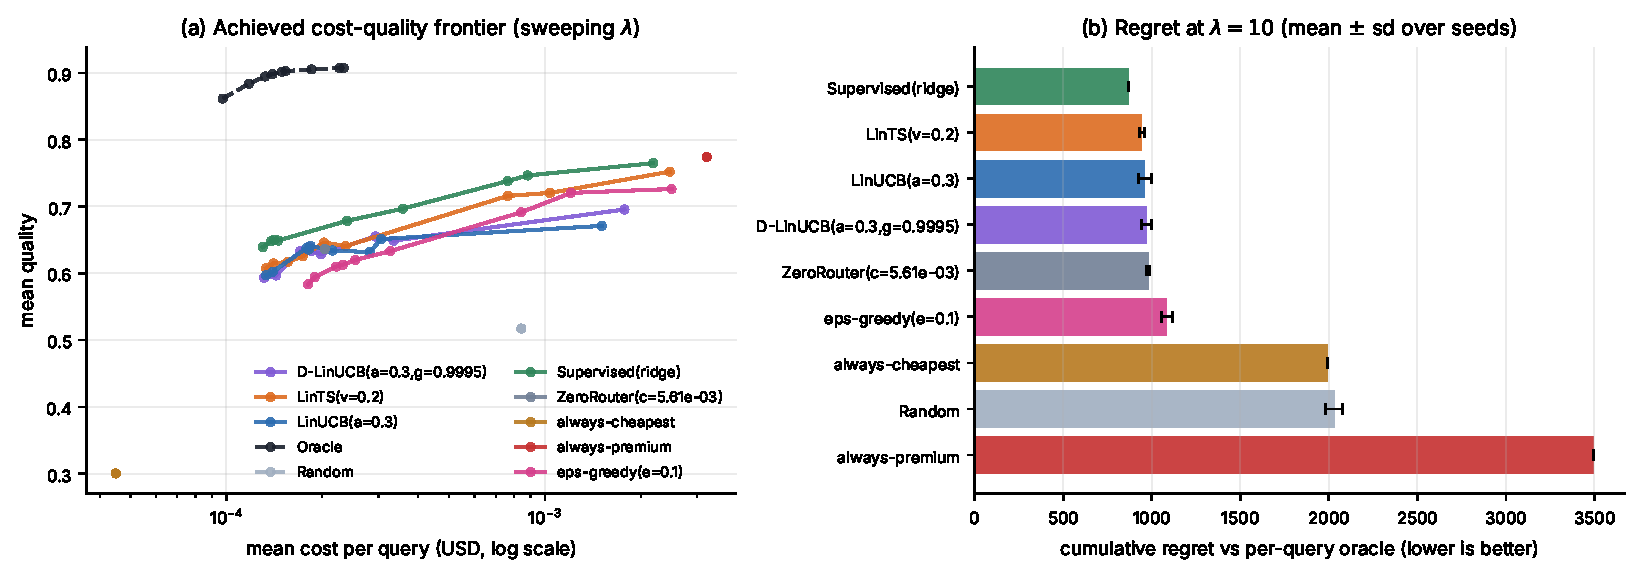
\includegraphics[width=0.92\textwidth]{fig4_rq1_frontier_regret.pdf}
\caption{RQ1. (a) Achieved cost--quality frontier as $\lam$ sweeps. (b)
Cumulative regret at $\lam=10$, mean $\pm$ sd over five seeds.}
\label{fig:rq1}
\end{figure*}

\begin{figure}[t]
\centering
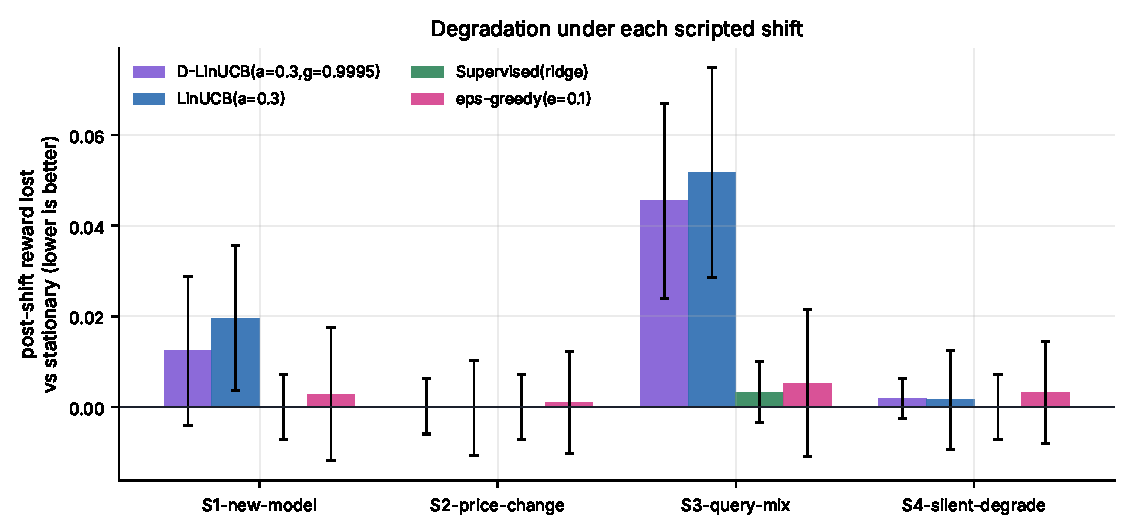
\includegraphics[width=\columnwidth]{fig5_rq2_shifts.pdf}
\caption{RQ2. Post-shift reward lost versus stationary. Only S1 and S3 produce
measurable effects; the supervised router is the most robust.}
\label{fig:rq2}
\end{figure}

\begin{figure}[t]
\centering
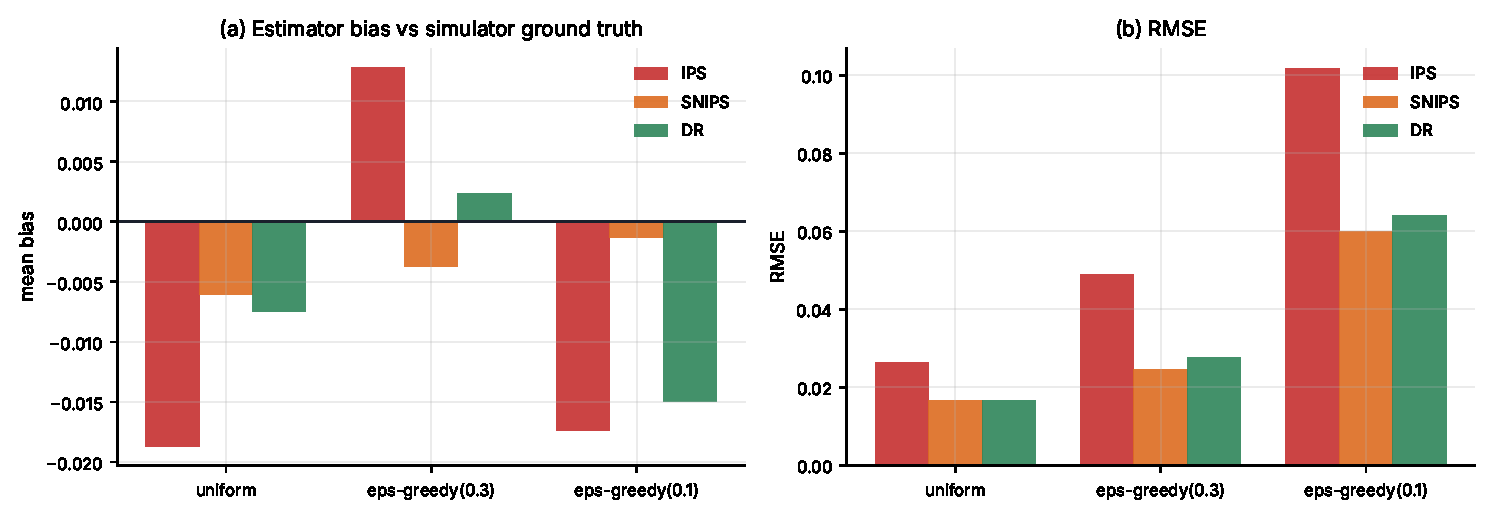
\includegraphics[width=\columnwidth]{fig6_rq3_ope.pdf}
\caption{OPE accuracy. IPS degrades sharply as logging propensities shrink;
SNIPS and DR remain stable.}
\label{fig:rq3}
\end{figure}

\section{Frameworks and Libraries}

Python 3.12 managed by \texttt{uv} with a committed lockfile, so
\texttt{uv sync \&\& uv run pytest} reproduces the environment exactly. The core
package depends only on NumPy, SciPy, scikit-learn, pandas and Matplotlib;
PyTorch and \texttt{sentence-transformers} sit in an optional \texttt{embed}
extra and HuggingFace clients in a \texttt{data} extra, both needed only for
one-time offline jobs. This keeps the install light for collaborators who only
run experiments. CI runs \texttt{ruff} and the test suite on every push.
Bandit policies, the environment, and the OPE estimators are our own
implementations; OBP is used only for cross-validation, as explained above.

\section{Revised Plan and Risks}

Remaining work, in priority order: (1) re-run everything at full scale
(36{,}497 queries); (2) make S2 and S4 bite, or report that RouterBench cannot
support them; (3) replace the recovery-time metric; (4) add the
sentence-transformer feature backend and compare; (5) implement PILOT as a SoTA
comparison; (6) sweep the Zero Router's target cost so it traces a full frontier
rather than a point.

The principal risk is now clearer than at proposal time. Our RQ2 hypothesis is
not currently supported: the static supervised router is more robust than the
bandits under every shift we can make bite. If that survives full-scale
replication, the honest contribution becomes a negative result---a
characterisation of when adaptive routing does \emph{not} pay---together with
the simulator, the calibration methodology, and the OPE validation, all of which
stand independently.

\begin{thebibliography}{99}\small
\bibitem[Agrawal \& Goyal(2013)]{agrawal2013thompson} S.~Agrawal and N.~Goyal.
Thompson sampling for contextual bandits with linear payoffs. \emph{ICML}, 2013.
\bibitem[Chen et al.(2023)]{chen2023frugalgpt} L.~Chen, M.~Zaharia, and J.~Zou.
FrugalGPT. \emph{arXiv:2305.05176}, 2023.
\bibitem[Dud\'ik et al.(2011)]{dudik2011doubly} M.~Dud\'ik, J.~Langford, and
L.~Li. Doubly robust policy evaluation and learning. \emph{ICML}, 2011.
\bibitem[Hu et al.(2024)]{hu2024routerbench} Q.~J.~Hu et al. RouterBench: a
benchmark for multi-LLM routing systems. \emph{arXiv:2403.12031}, 2024.
\bibitem[Li et al.(2010)]{li2010contextual} L.~Li, W.~Chu, J.~Langford, and
R.~E. Schapire. A contextual-bandit approach to personalized news article
recommendation. \emph{WWW}, 2010.
\bibitem[Lu et al.(2026)]{lu2026routerarena} Y.~Lu et al. RouterArena: an open
platform for comprehensive comparison of LLM routers. \emph{ICLR}, 2026.
\bibitem[Ong et al.(2025)]{ong2025routellm} I.~Ong et al. RouteLLM: learning to
route LLMs with preference data. \emph{ICLR}, 2025.
\bibitem[Panda et al.(2025)]{panda2025adaptive} P.~Panda, R.~Magazine,
C.~Devaguptapu, S.~Takemori, and V.~Sharma. Adaptive LLM routing under budget
constraints. \emph{Findings of EMNLP}, 2025.
\bibitem[Russac et al.(2019)]{russac2019weighted} Y.~Russac, C.~Vernade, and
O.~Capp\'e. Weighted linear bandits for non-stationary environments.
\emph{NeurIPS}, 2019.
\bibitem[Saito et al.(2021)]{saito2021open} Y.~Saito, S.~Aihara, M.~Matsutani,
and Y.~Narita. Open bandit dataset and pipeline. \emph{NeurIPS D\&B}, 2021.
\bibitem[Taberner-Miller(2026)]{taberner2026pareto} A.~Taberner-Miller.
ParetoBandit: budget-paced adaptive routing for non-stationary LLM serving.
\emph{arXiv:2604.00136}, 2026.
\bibitem[Wei et al.(2025)]{wei2025bandit} W.~Wei et al. Learning to route LLMs
from bandit feedback: one policy, many trade-offs. \emph{arXiv:2510.07429},
2025.
\end{thebibliography}

\end{document}
